\begin{figure}
\centering
\begin{minipage}{.5\textwidth}
  \captionof{figure}{Baroque Period}
  \centering
  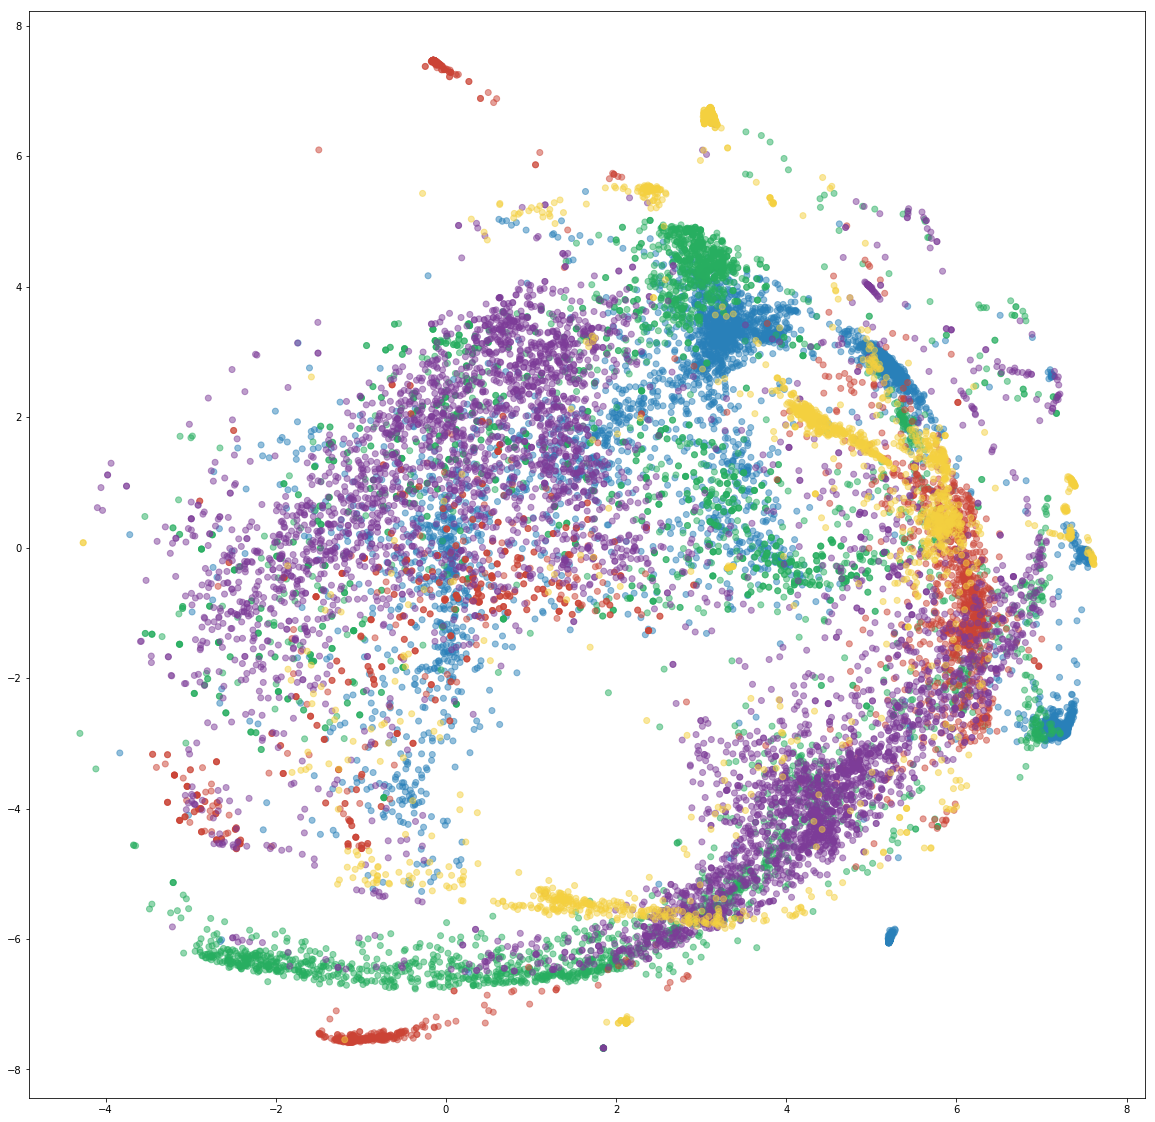
\includegraphics[scale=0.15]{era1}
  \label{fig:test1}
\end{minipage}%
\begin{minipage}{.5\textwidth}
  \captionof{figure}{Classical Period}
  \centering
  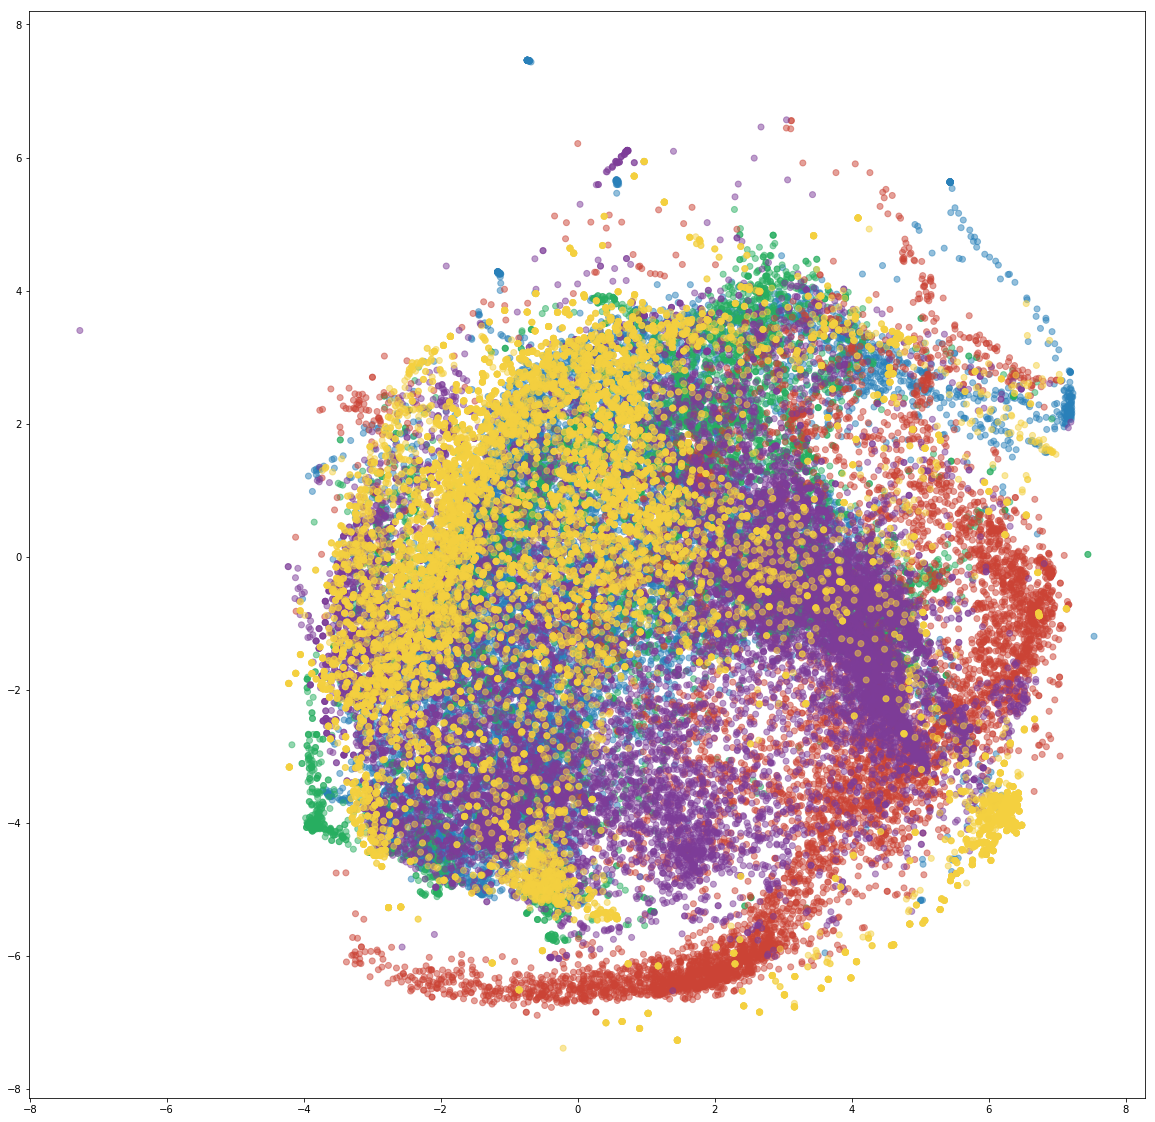
\includegraphics[scale=0.15]{era2}
  \label{fig:test2}
\end{minipage}
\end{figure}

\begin{figure}
\centering
\begin{minipage}{.5\textwidth}
  \captionof{figure}{19th Century}
  \centering
  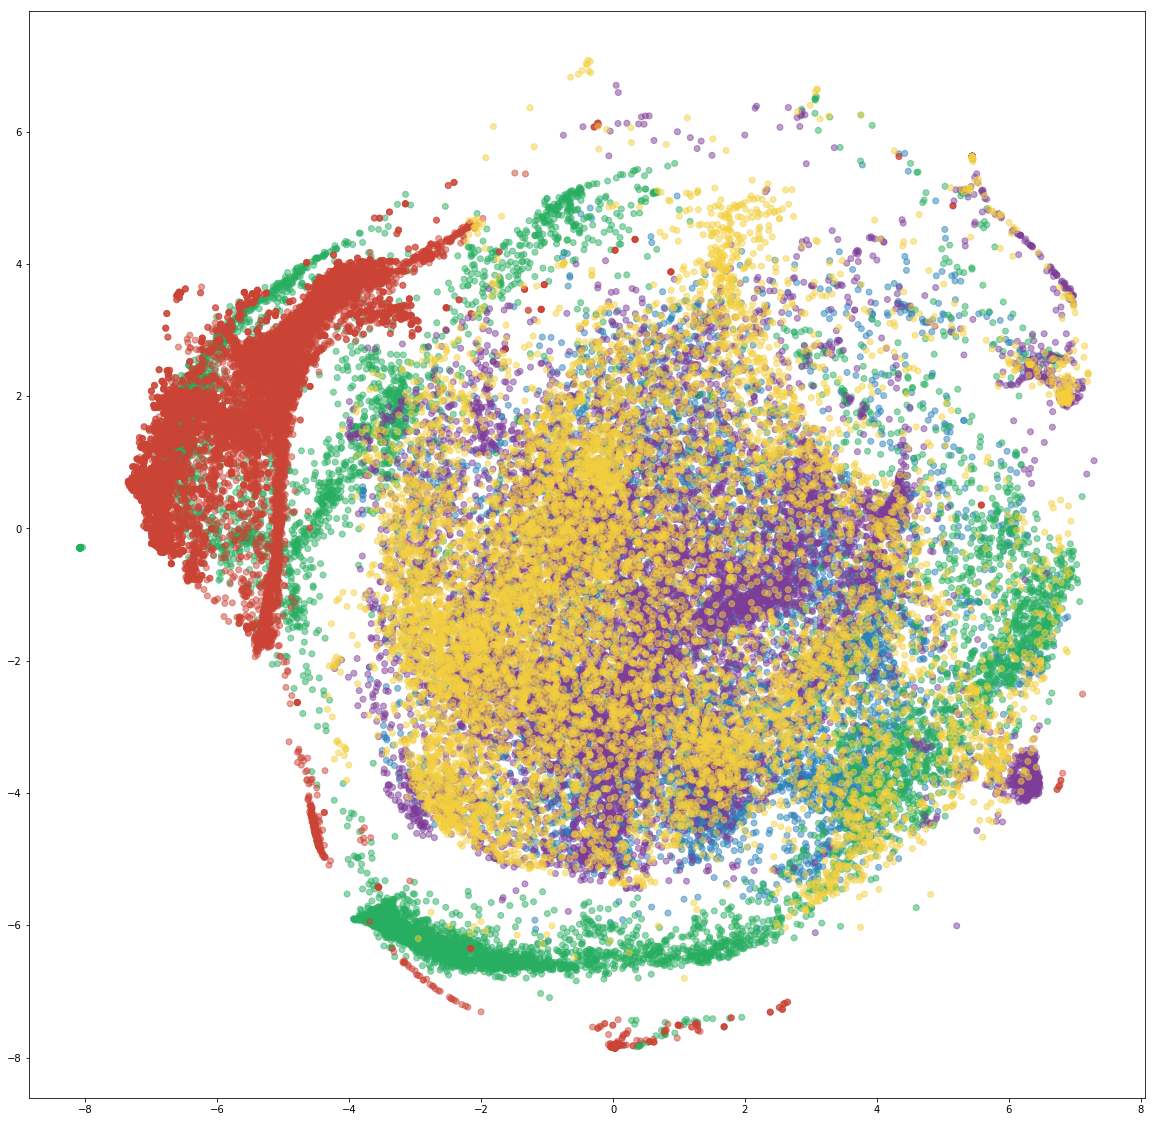
\includegraphics[scale=0.15]{era3}
  \label{fig:test1}
\end{minipage}%
\begin{minipage}{.5\textwidth}
  \captionof{figure}{Romantic Period}
  \centering
  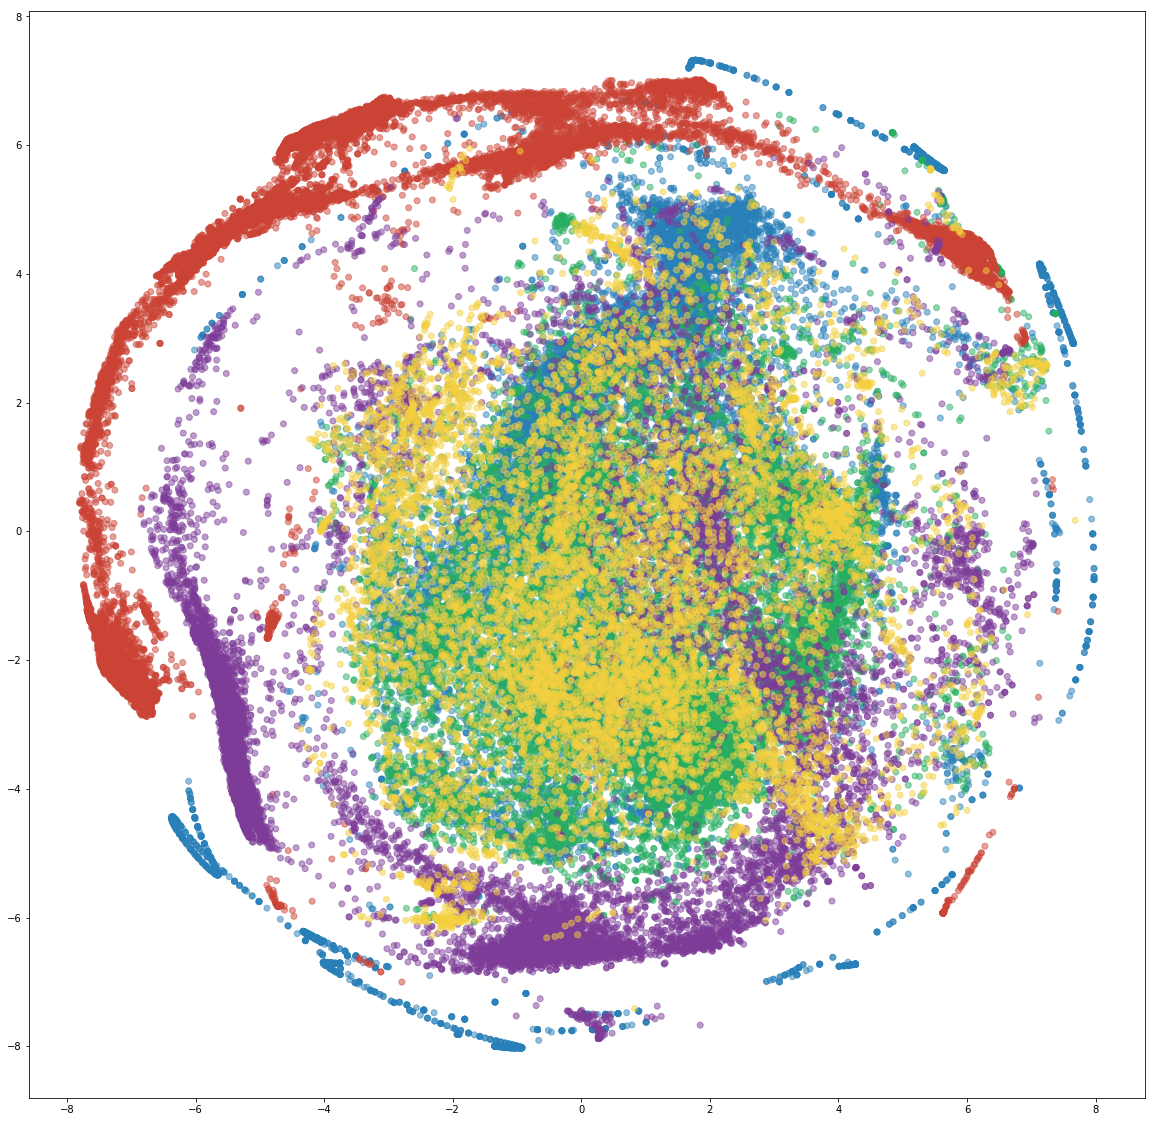
\includegraphics[scale=0.15]{era4}
  \label{fig:test2}
\end{minipage}
\end{figure}

\begin{figure}[h]
\caption{20th Century}
\centering
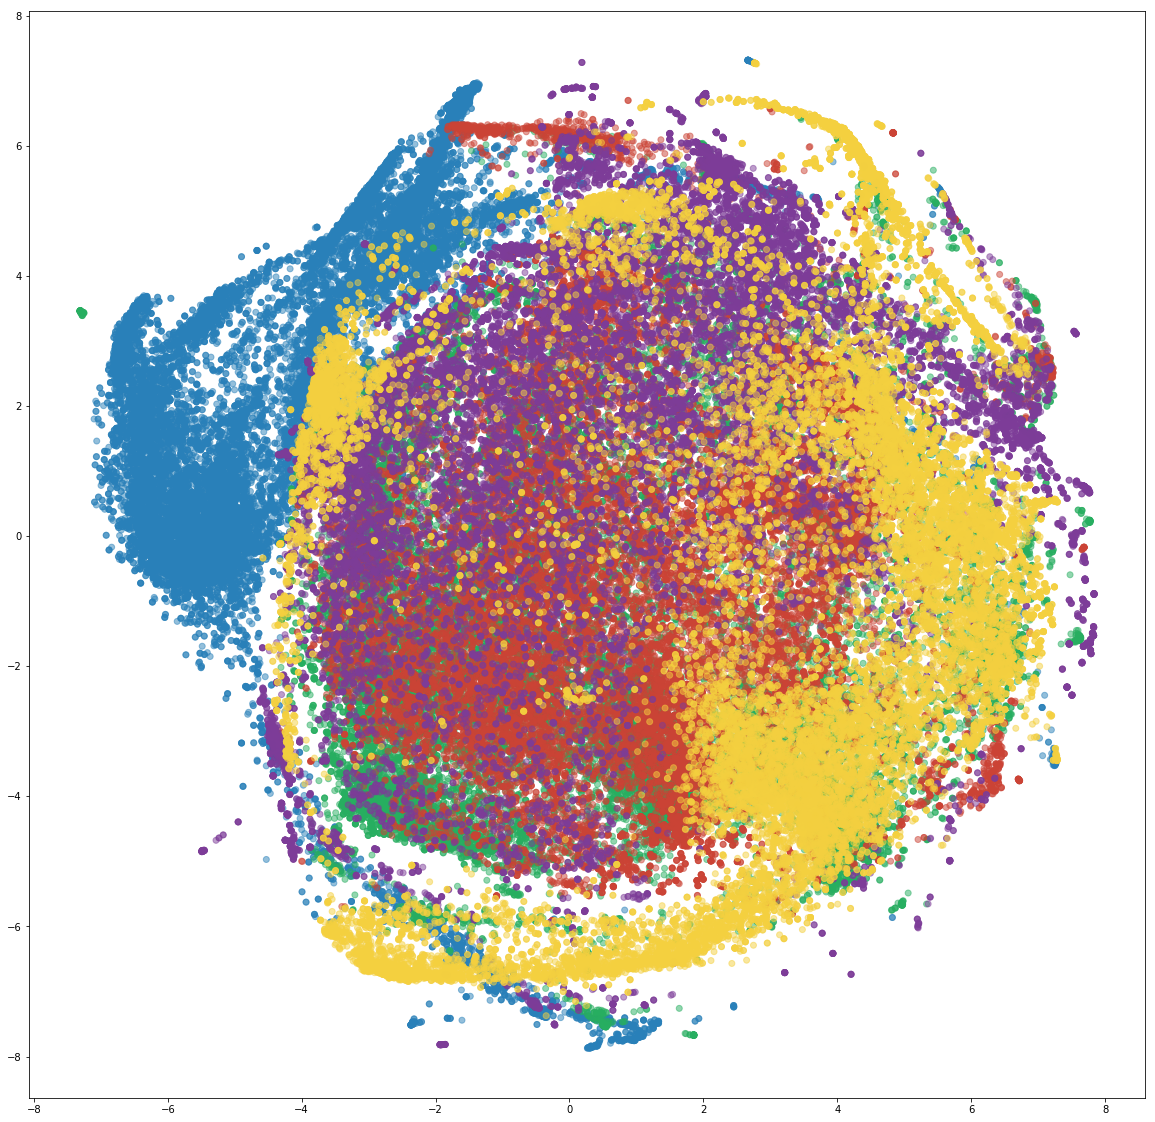
\includegraphics[scale=0.15]{era5}
\end{figure}

\begin{figure}
\centering
\begin{minipage}{.5\textwidth}
  \captionof{figure}{Baroque: Bach}
  \centering
  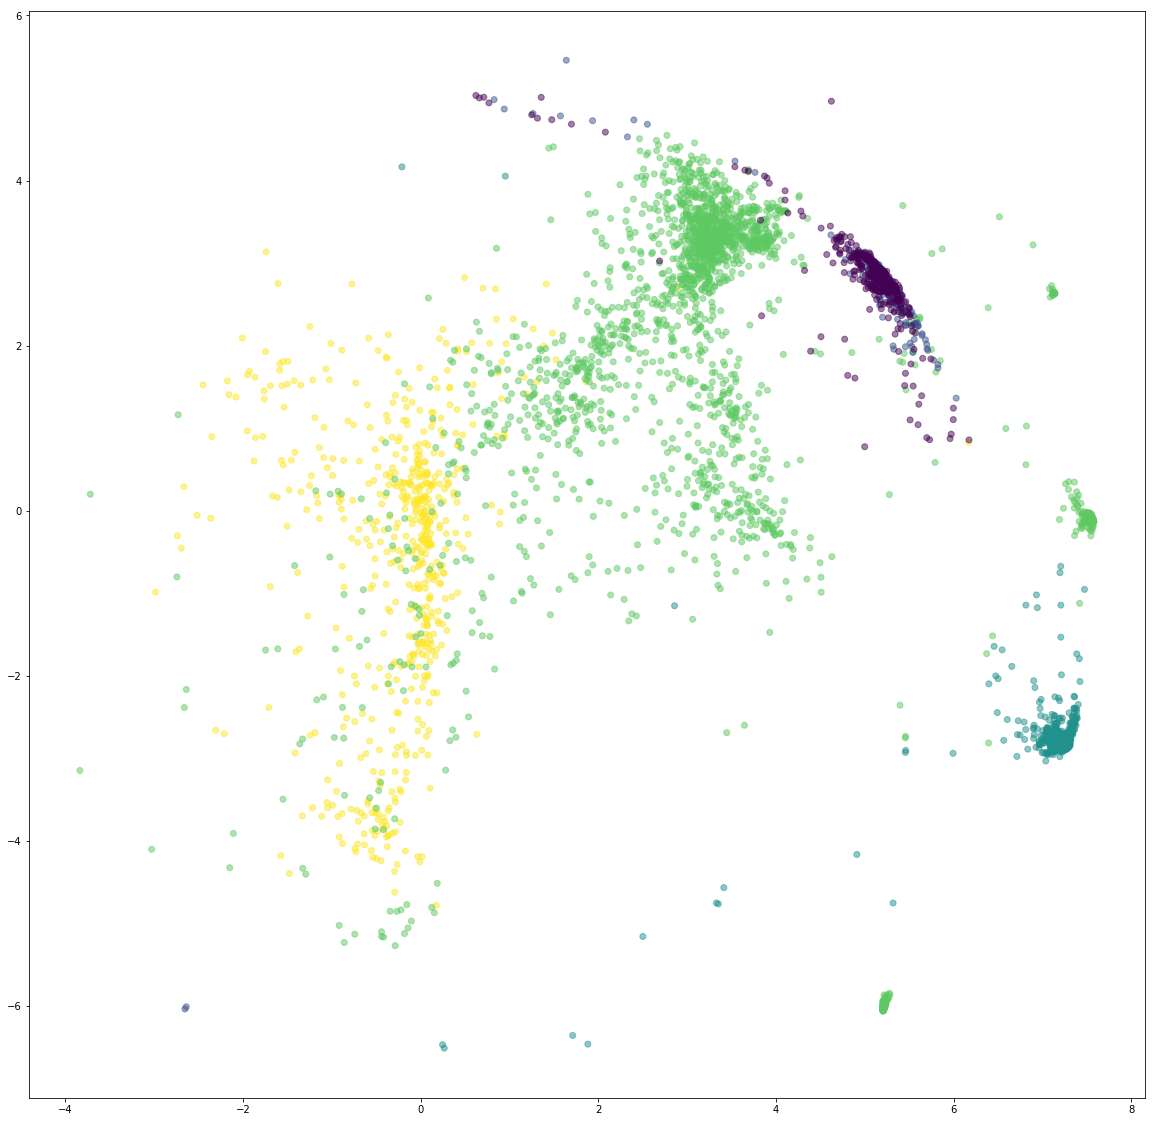
\includegraphics[scale=0.15]{P1C1}
  \label{fig:test1}
\end{minipage}%
\begin{minipage}{.5\textwidth}
  \captionof{figure}{Baroque: Boyce}
  \centering
  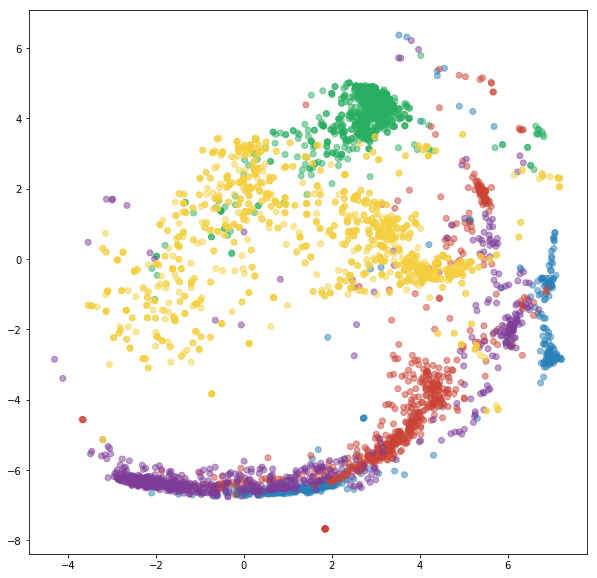
\includegraphics[scale=0.15]{P1C2}
  \label{fig:test2}
\end{minipage}
\end{figure}

\begin{figure}
\centering
\begin{minipage}{.5\textwidth}
  \captionof{figure}{Baroque: Gabrieli}
  \centering
  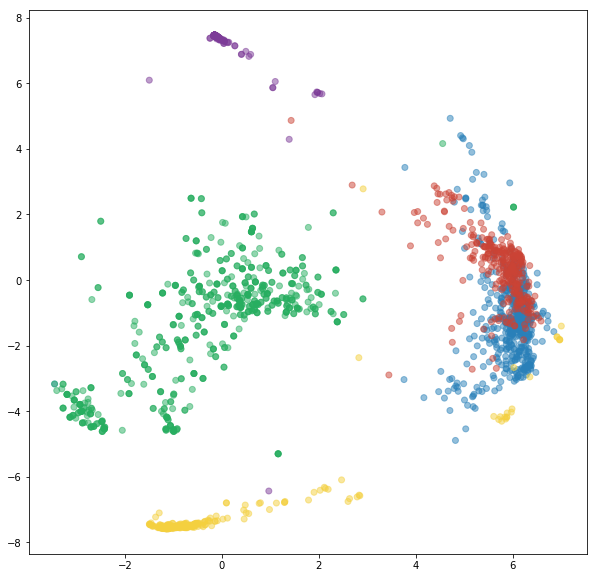
\includegraphics[scale=0.15]{P1C3}
  \label{fig:test1}
\end{minipage}%
\begin{minipage}{.5\textwidth}
  \captionof{figure}{Baroque: Sammartini}
  \centering
  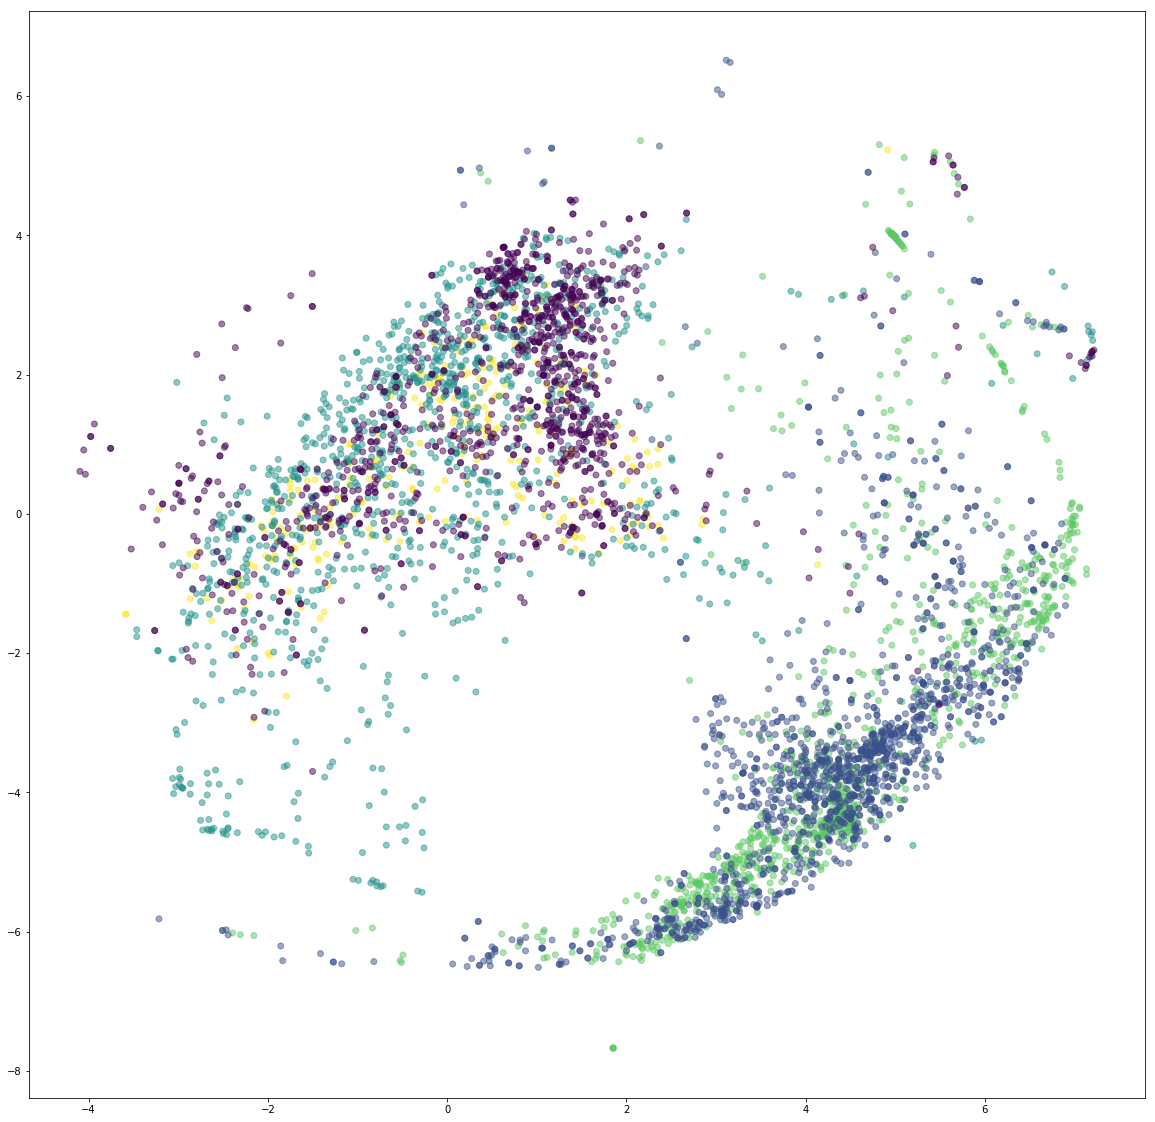
\includegraphics[scale=0.15]{P1C4}
  \label{fig:test2}
\end{minipage}
\end{figure}

\begin{figure}[h]
\caption{Baroque: Viadana}
\centering
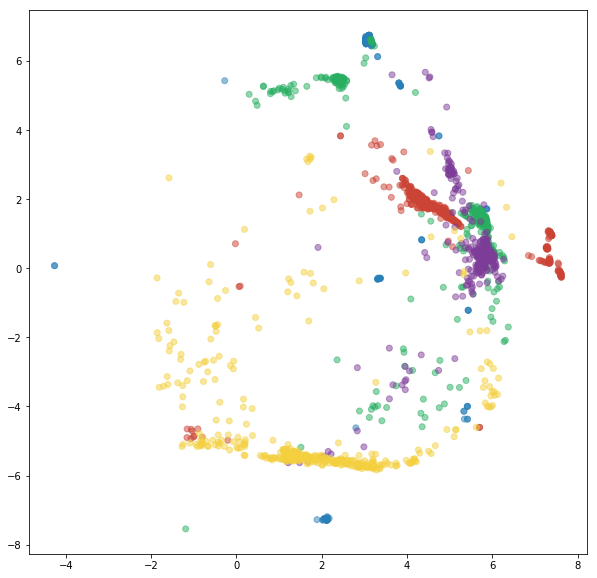
\includegraphics[scale=0.15]{P1C5}
\end{figure}

\begin{figure}
\centering
\begin{minipage}{.5\textwidth}
  \captionof{figure}{Classical: Boccherini}
  \centering
  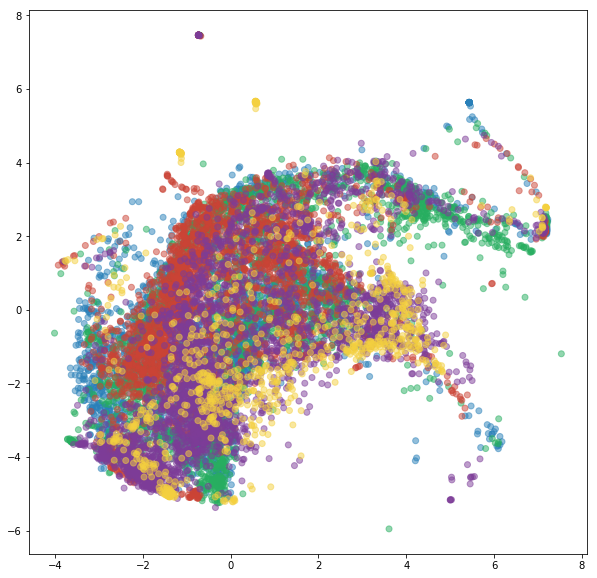
\includegraphics[scale=0.15]{P2C1}
  \label{fig:test1}
\end{minipage}%
\begin{minipage}{.5\textwidth}
  \captionof{figure}{Classical: Gluck}
  \centering
  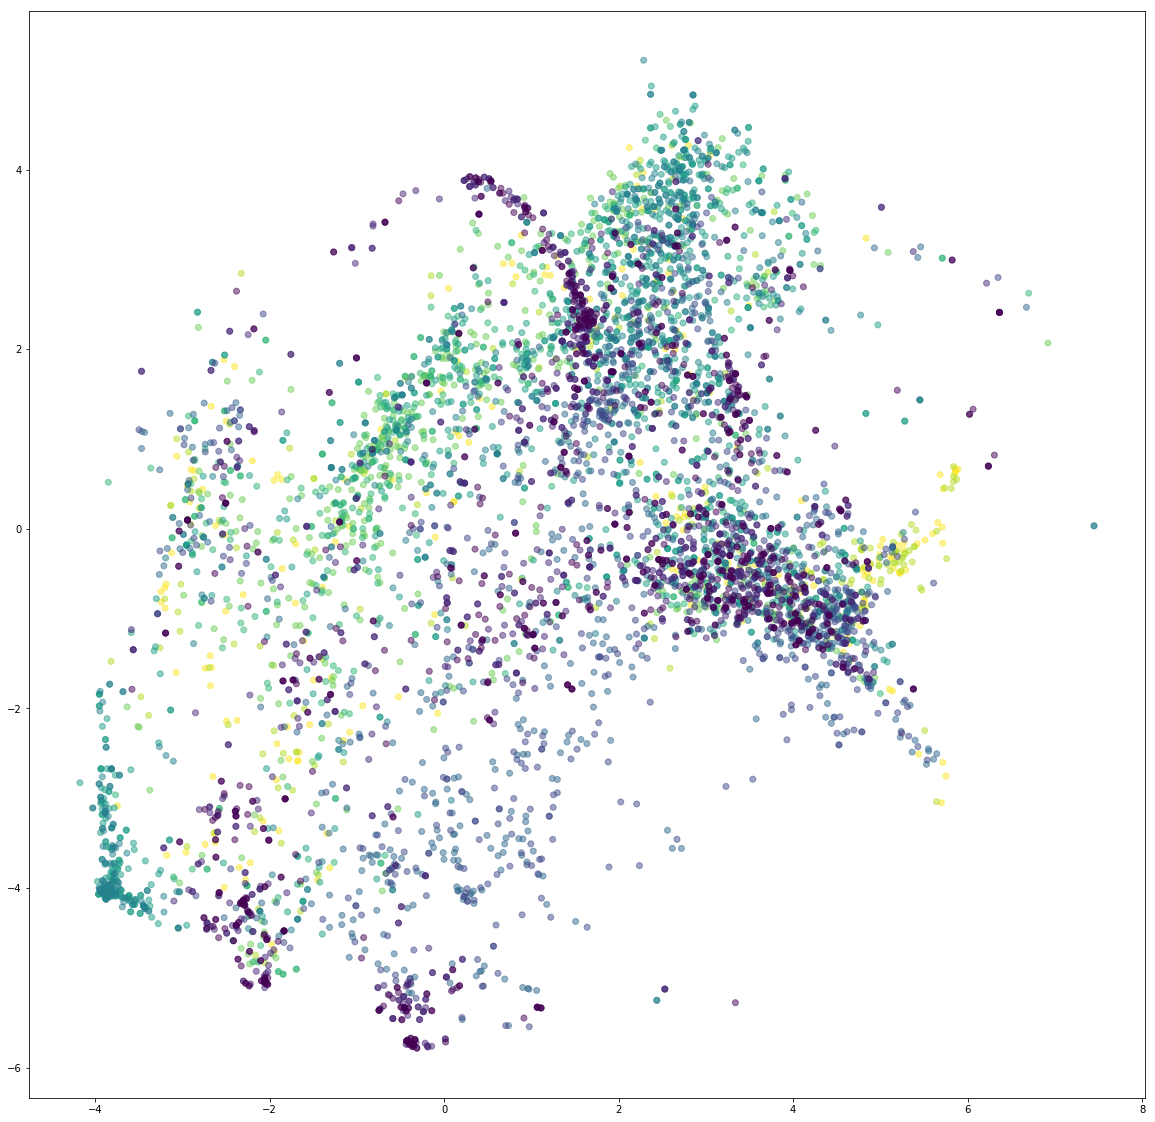
\includegraphics[scale=0.15]{P2C2}
  \label{fig:test2}
\end{minipage}
\end{figure}

\begin{figure}
\centering
\begin{minipage}{.5\textwidth}
  \captionof{figure}{Classical: Haydn}
  \centering
  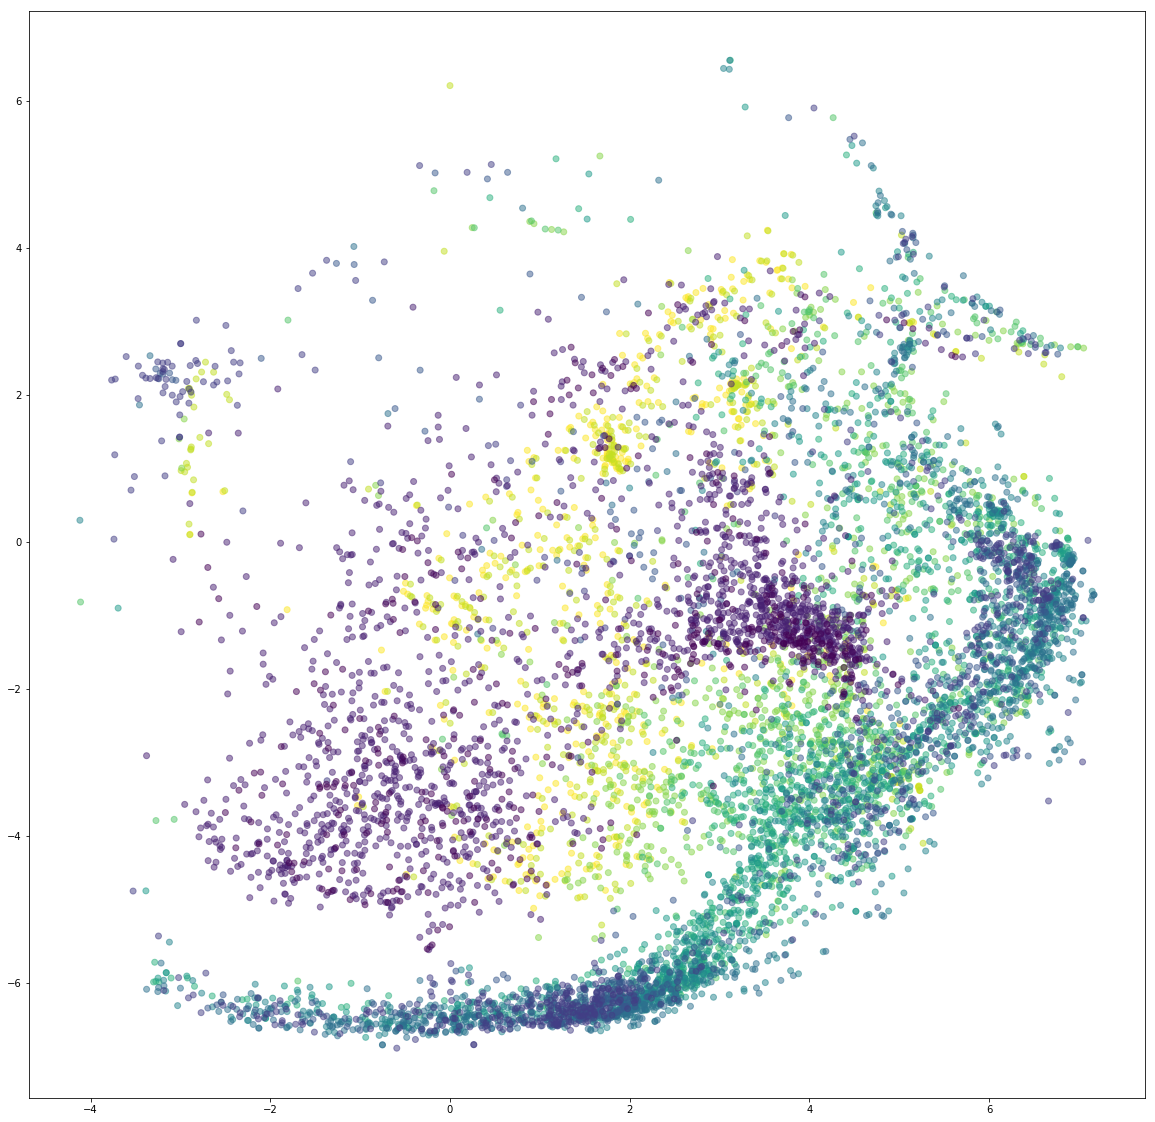
\includegraphics[scale=0.15]{P2C3}
  \label{fig:test1}
\end{minipage}%
\begin{minipage}{.5\textwidth}
  \captionof{figure}{Classical: Mozart}
  \centering
  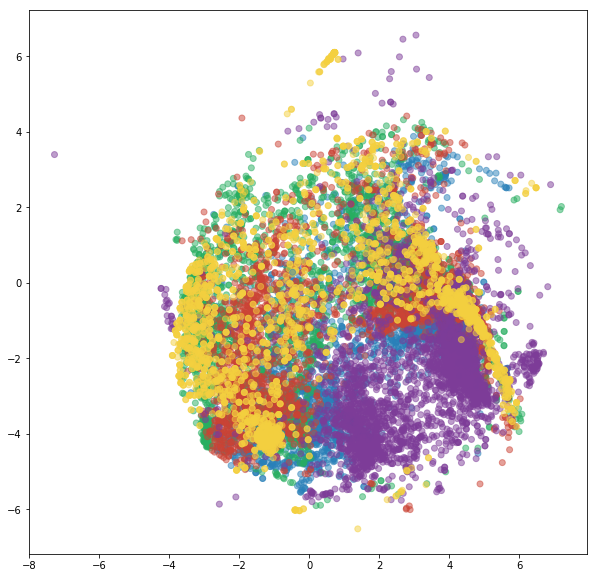
\includegraphics[scale=0.15]{P2C4}
  \label{fig:test2}
\end{minipage}
\end{figure}

\begin{figure}[h]
\caption{Classical: Salieri}
\centering
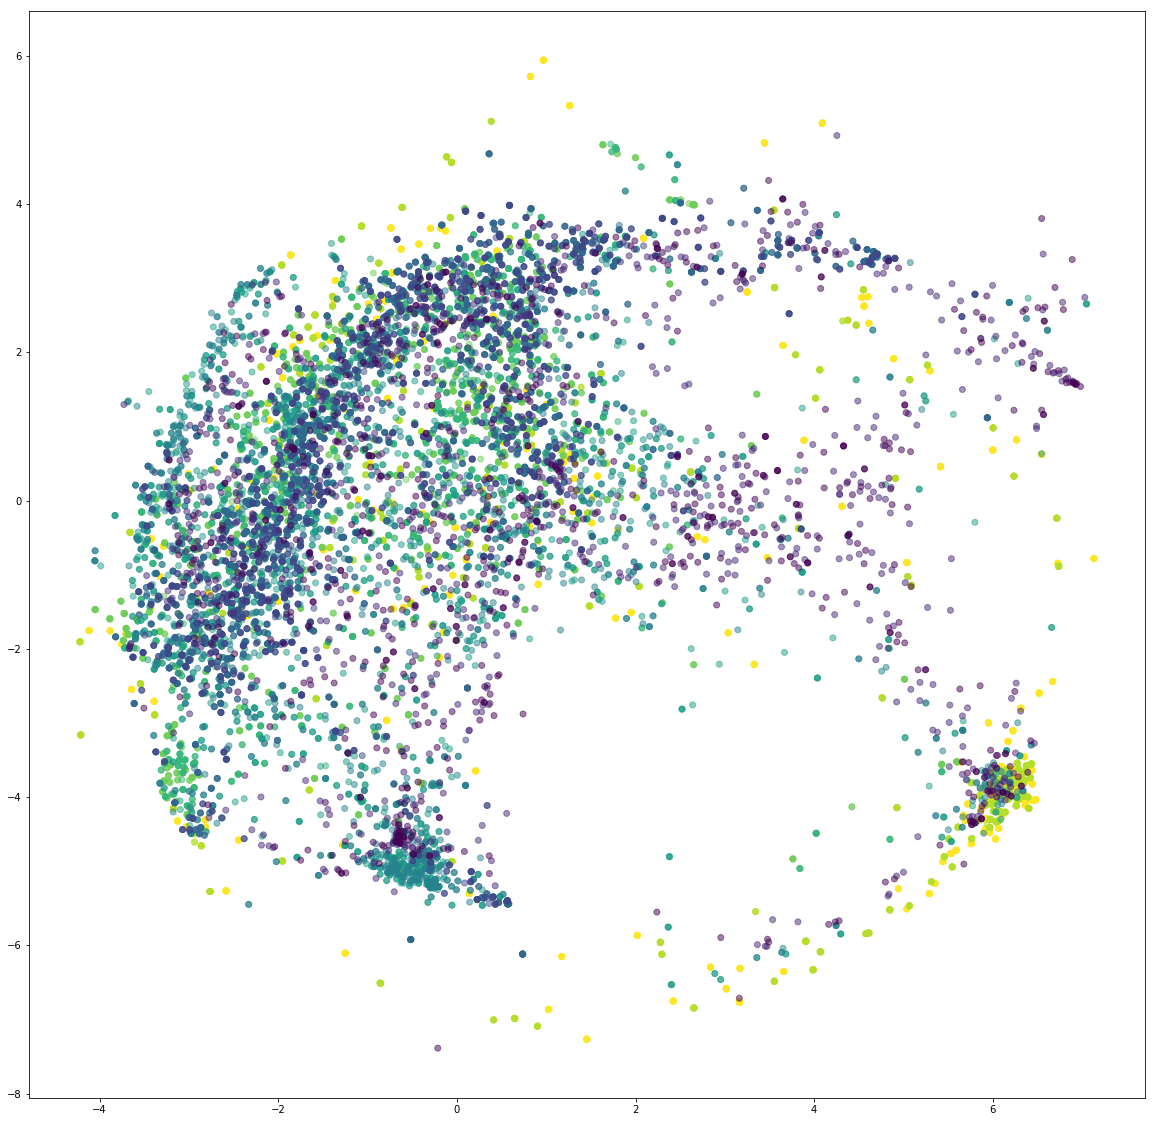
\includegraphics[scale=0.15]{P2C5}
\end{figure}

\begin{figure}
\centering
\begin{minipage}{.5\textwidth}
  \captionof{figure}{19th Century: Beethoven}
  \centering
  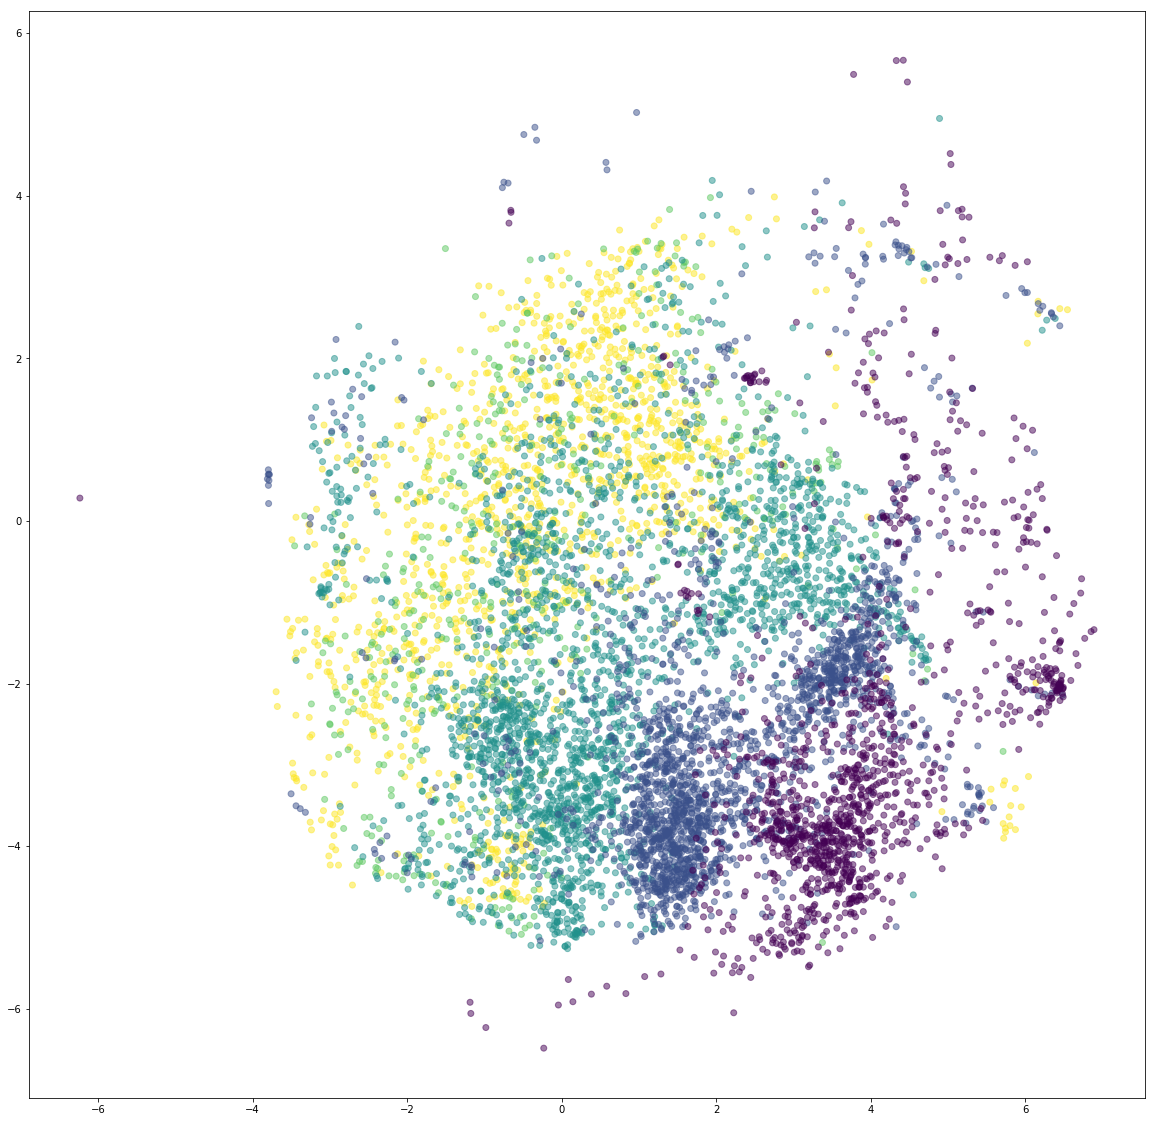
\includegraphics[scale=0.15]{P3C1}
  \label{fig:test1}
\end{minipage}%
\begin{minipage}{.5\textwidth}
  \captionof{figure}{19th Century: Clementi}
  \centering
  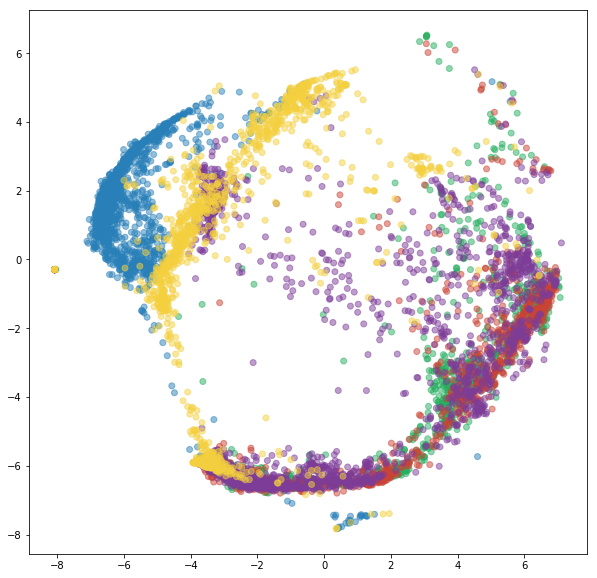
\includegraphics[scale=0.15]{P3C2}
  \label{fig:test2}
\end{minipage}
\end{figure}

\begin{figure}
\centering
\begin{minipage}{.5\textwidth}
  \captionof{figure}{19th Century: Gossec}
  \centering
  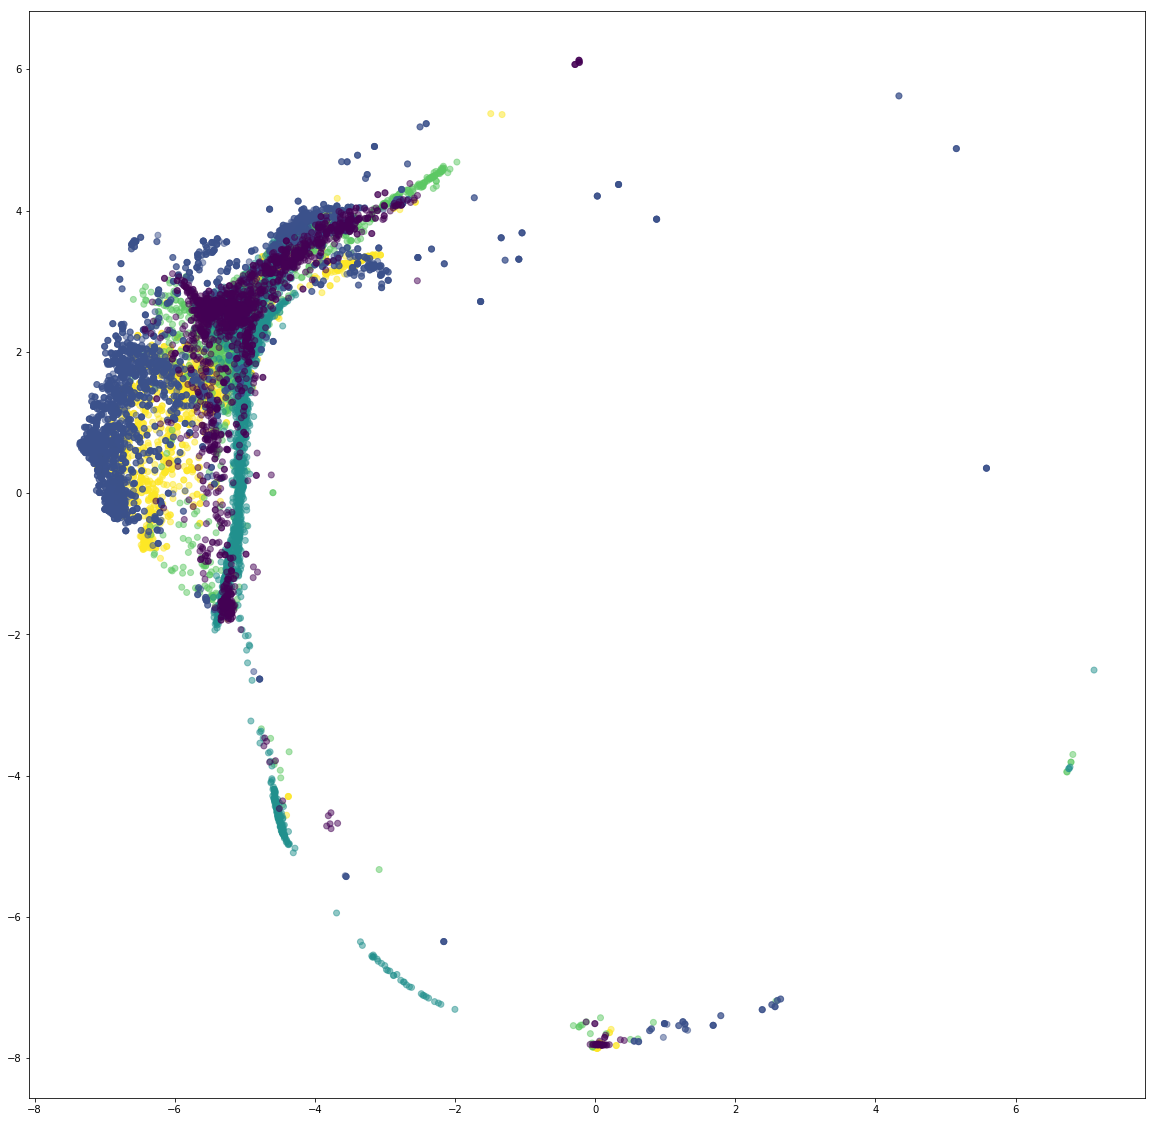
\includegraphics[scale=0.15]{P3C3}
  \label{fig:test1}
\end{minipage}%
\begin{minipage}{.5\textwidth}
  \captionof{figure}{19th Century: Kalliwoda}
  \centering
  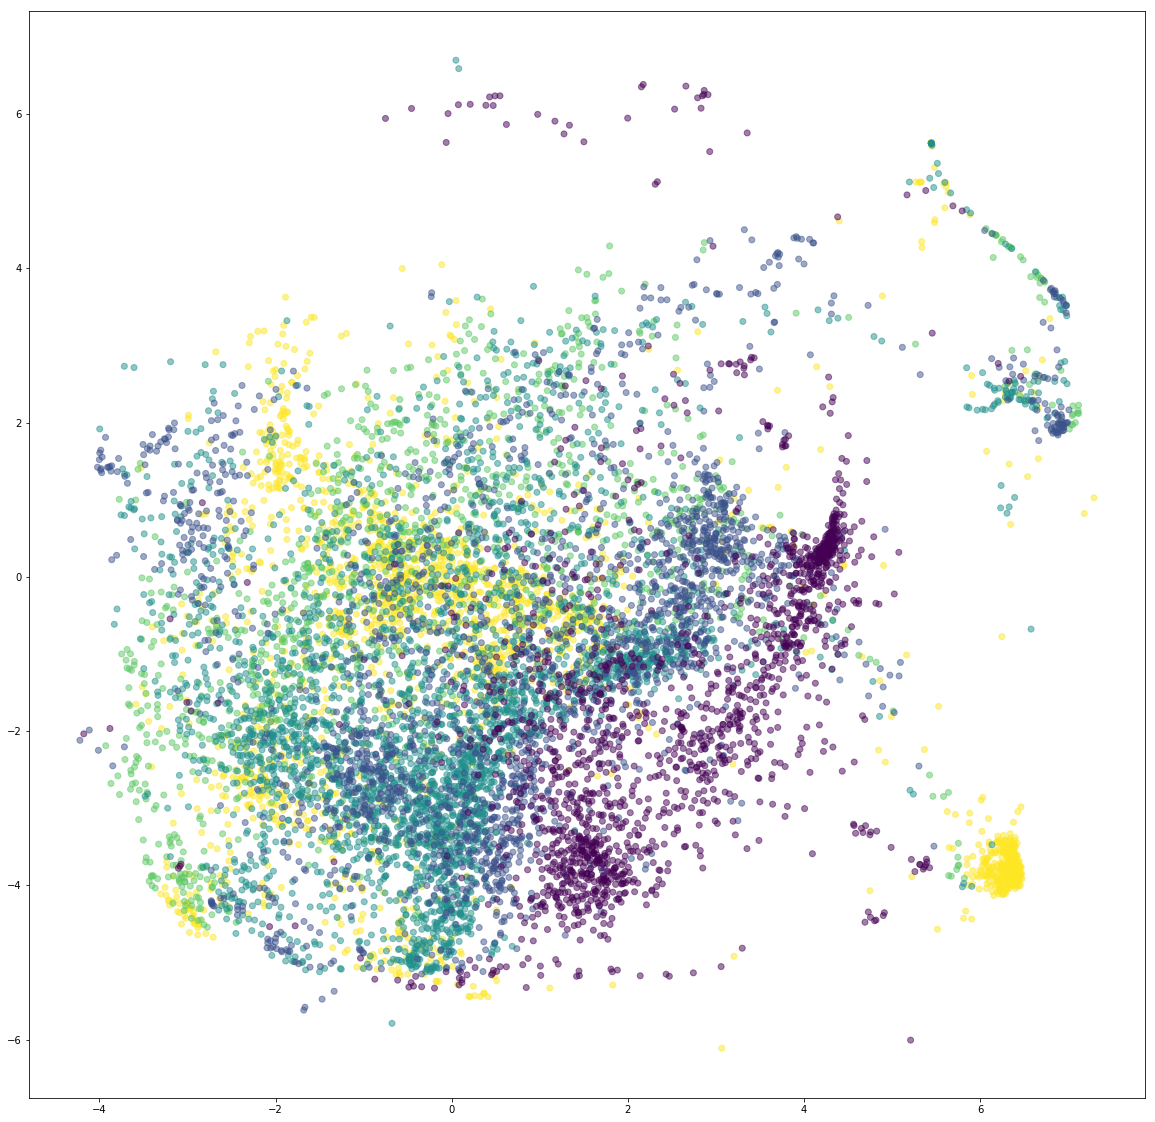
\includegraphics[scale=0.15]{P3C4}
  \label{fig:test2}
\end{minipage}
\end{figure}

\begin{figure}[h]
\caption{19th Century: Rubinstein}
\centering
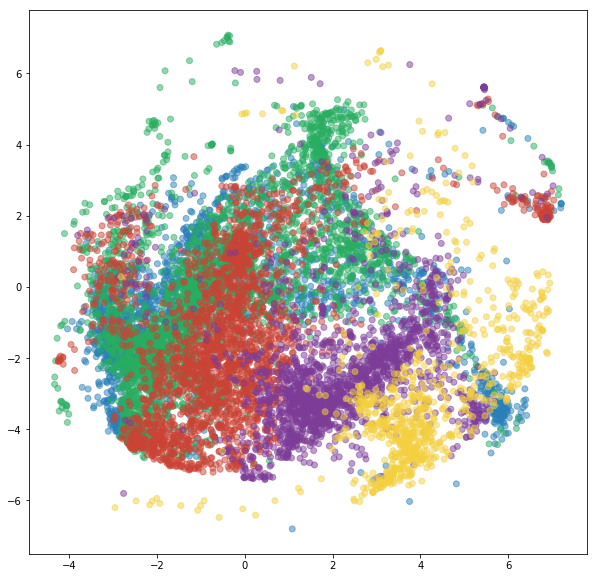
\includegraphics[scale=0.15]{P3C5}
\end{figure}

\begin{figure}
\centering
\begin{minipage}{.5\textwidth}
  \captionof{figure}{Romantic: Dvorak}
  \centering
  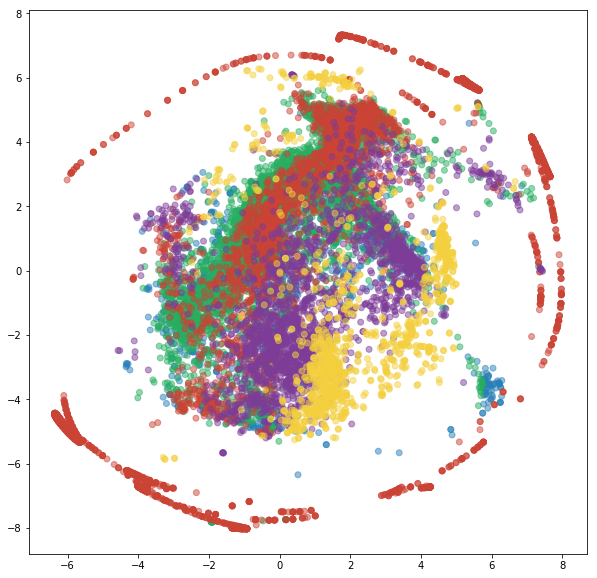
\includegraphics[scale=0.15]{P4C1}
  \label{fig:test1}
\end{minipage}%
\begin{minipage}{.5\textwidth}
  \captionof{figure}{Romantic: Mendelssohn}
  \centering
  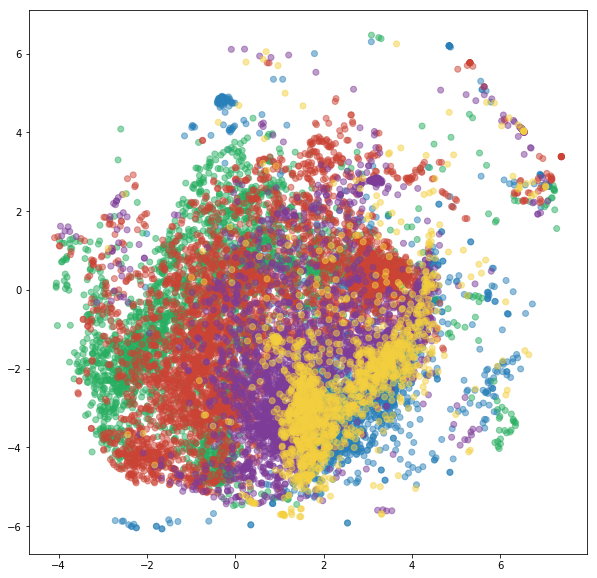
\includegraphics[scale=0.15]{P4C2}
  \label{fig:test2}
\end{minipage}
\end{figure}

\begin{figure}
\centering
\begin{minipage}{.5\textwidth}
  \captionof{figure}{Romantic: Schubert}
  \centering
  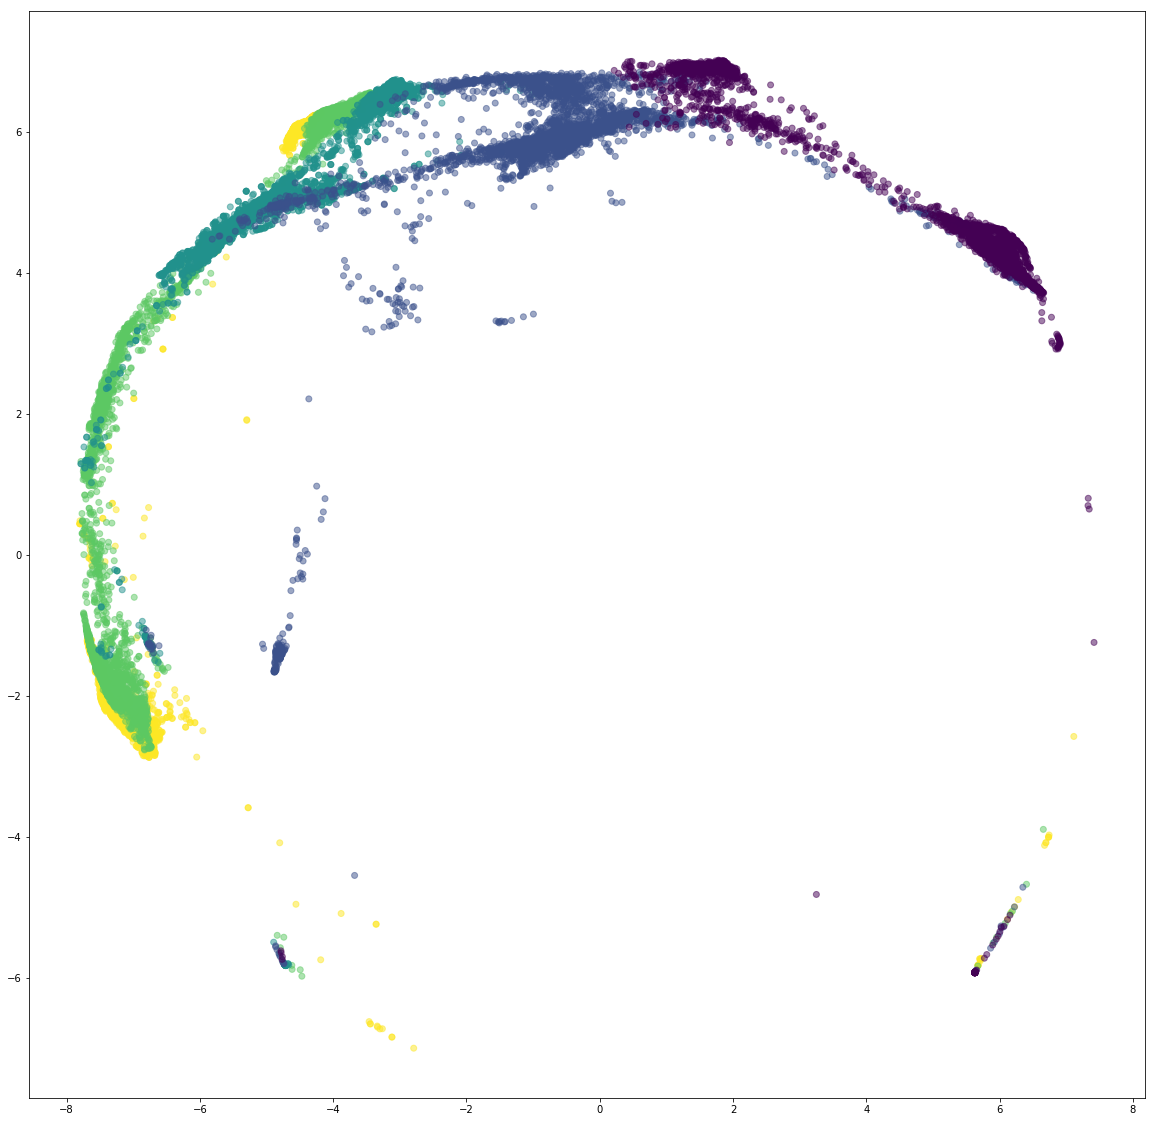
\includegraphics[scale=0.15]{P4C3}
  \label{fig:test1}
\end{minipage}%
\begin{minipage}{.5\textwidth}
  \captionof{figure}{Romantic: Schumann}
  \centering
  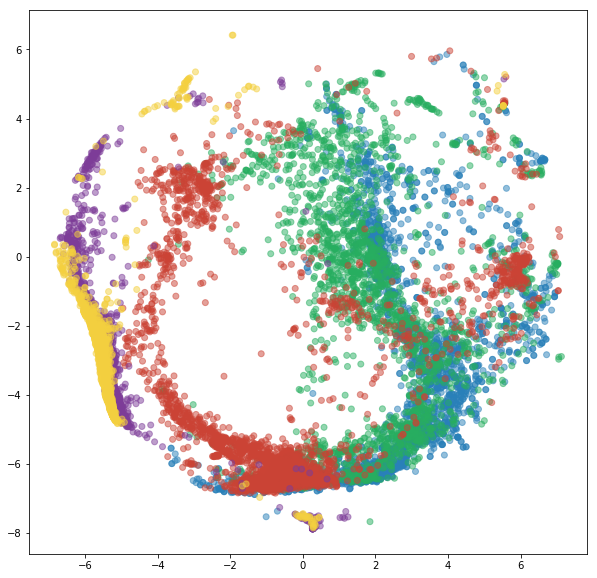
\includegraphics[scale=0.15]{P4C4}
  \label{fig:test2}
\end{minipage}
\end{figure}

\begin{figure}[h]
\caption{Romantic: Tchaikovsky}
\centering
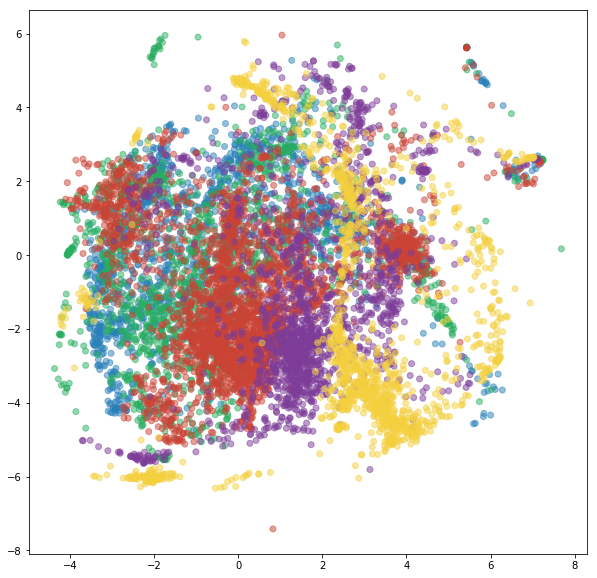
\includegraphics[scale=0.15]{P4C5}
\end{figure}

\begin{figure}
\centering
\begin{minipage}{.5\textwidth}
  \captionof{figure}{20th Cen: Antheil}
  \centering
  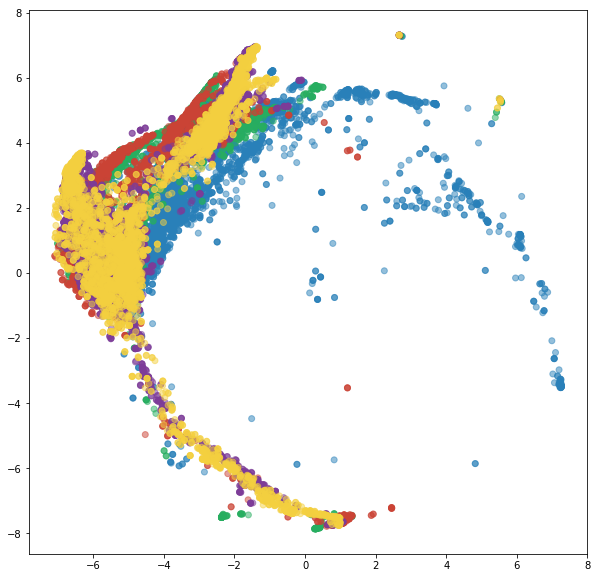
\includegraphics[scale=0.15]{P5C1}
  \label{fig:test1}
\end{minipage}%
\begin{minipage}{.5\textwidth}
  \captionof{figure}{20th Cen: Rachmaninoff}
  \centering
  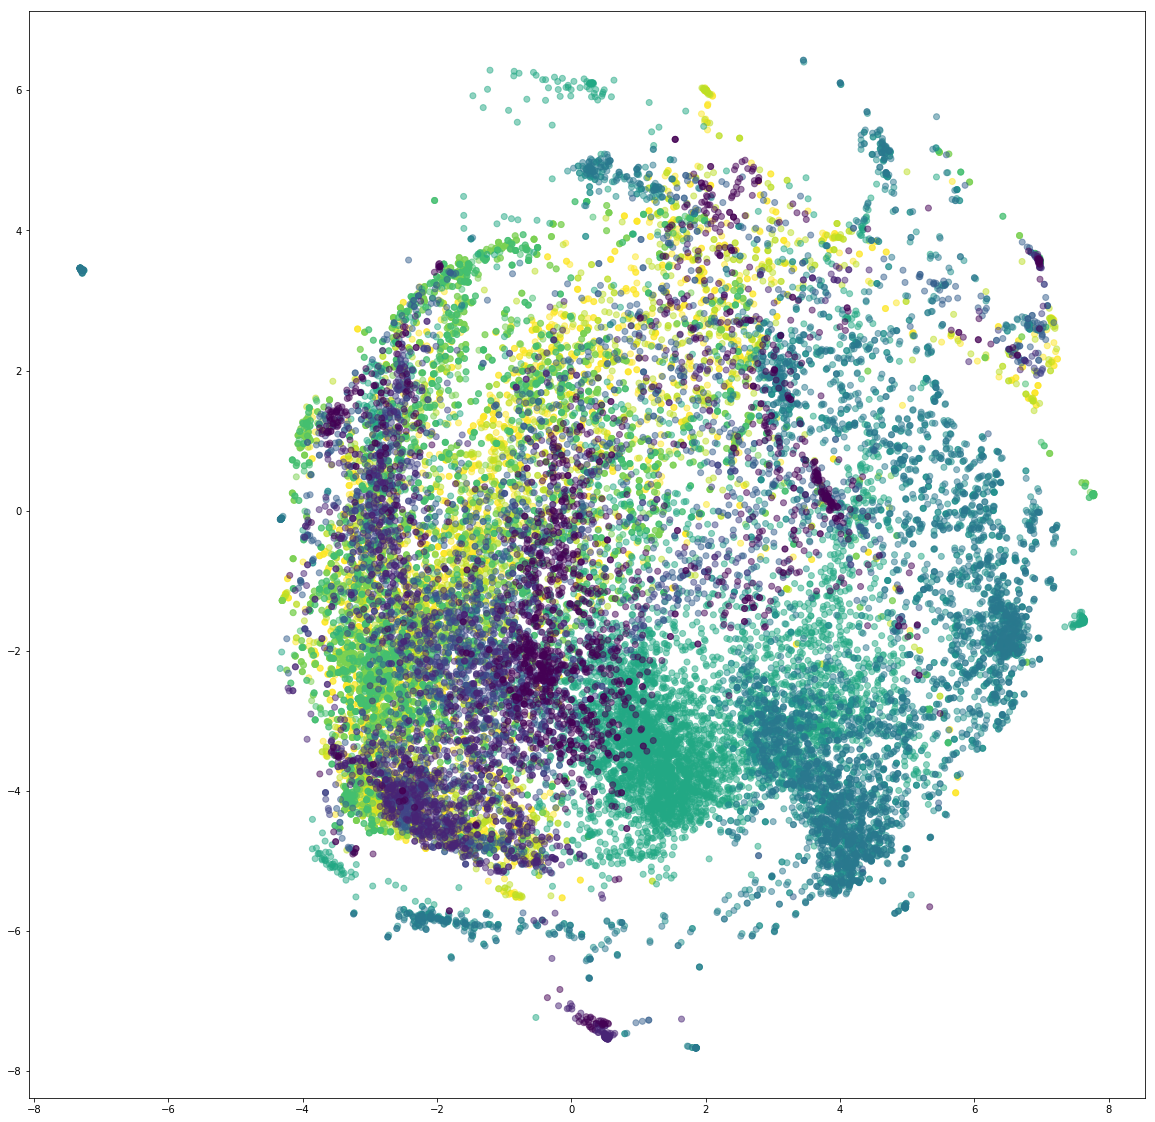
\includegraphics[scale=0.15]{P5C2}
  \label{fig:test2}
\end{minipage}
\end{figure}

\begin{figure}
\centering
\begin{minipage}{.5\textwidth}
  \captionof{figure}{20th Cen: Rubbra}
  \centering
  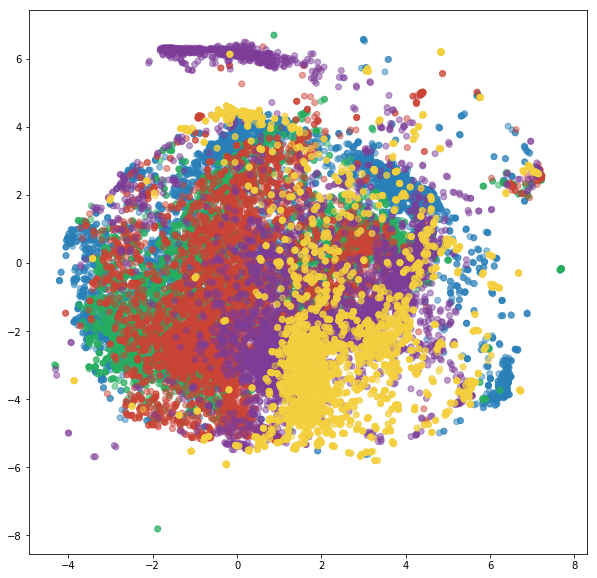
\includegraphics[scale=0.15]{P5C3}
  \label{fig:test1}
\end{minipage}%
\begin{minipage}{.5\textwidth}
  \captionof{figure}{20th Cen: Shostakovich}
  \centering
  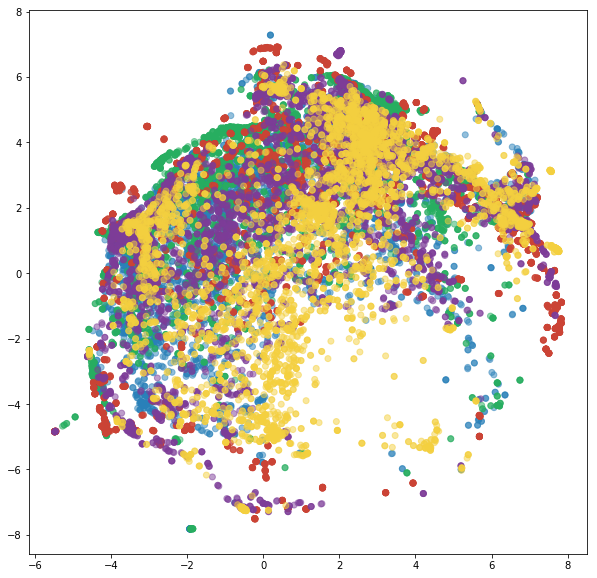
\includegraphics[scale=0.15]{P5C4}
  \label{fig:test2}
\end{minipage}
\end{figure}

\begin{figure}[h]
\caption{20th Cen: Stravinsky}
\centering
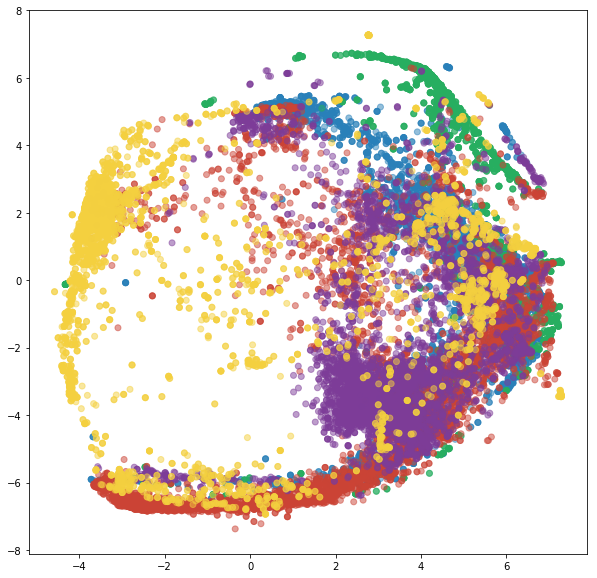
\includegraphics[scale=0.15]{P5C5}
\end{figure}